%------------------------------------------------------------------------------
%  web.tex
%------------------------------------------------------------------------------
%
%	BA6 - Database systems
%
%	Authors :
%		203267 - Bastien Antoine
%		183785 - Denoréaz Thomas
%		185078 - Dieulivol David
%
%	Versions :
%		2013.04.21 - Initial version
%

\chapter{Web}

\section{Entities \& relations}

Here is a view that show the listing of an entity or a relation, we can see that the SQL statement is above the table.
We can directly edit or remove an entry when clicking on the edit or delete link.

\begin{figure}[!ht]
	\centering
	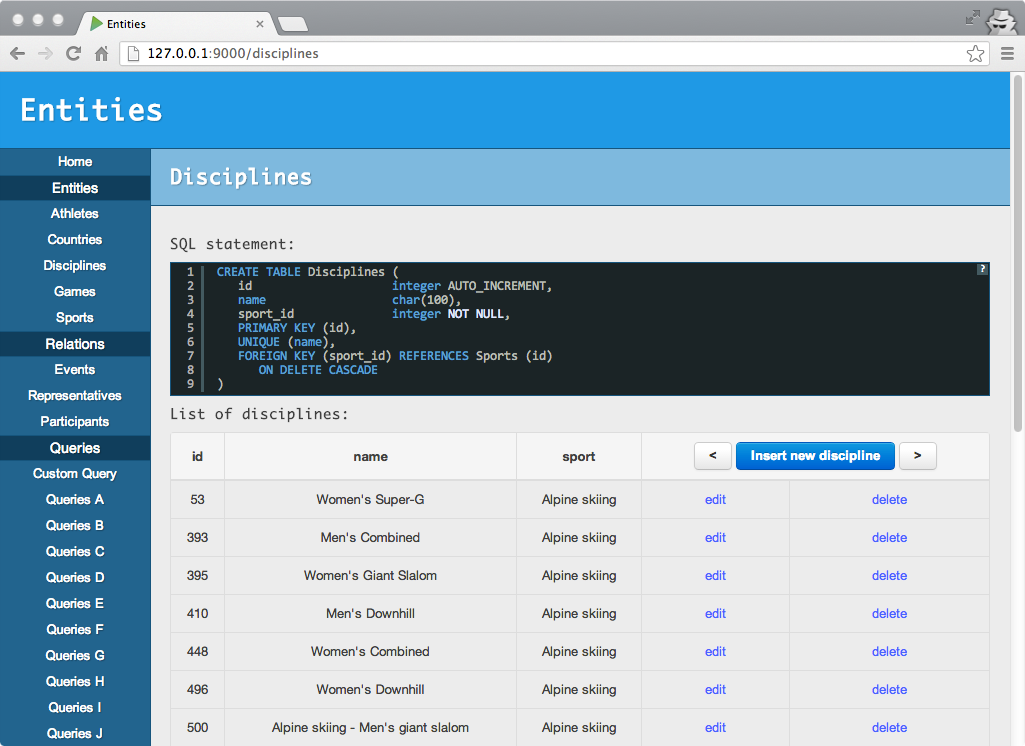
\includegraphics[width=0.9\textwidth]{web3_Entities}
	\caption{Entities listing\label{fig:ddl-scheme}}
\end{figure}

\newpage
\section{Query view}

The result of each query is shown inside a table, a description and the SQL statement are above the results.

\begin{figure}[!ht]
	\centering
	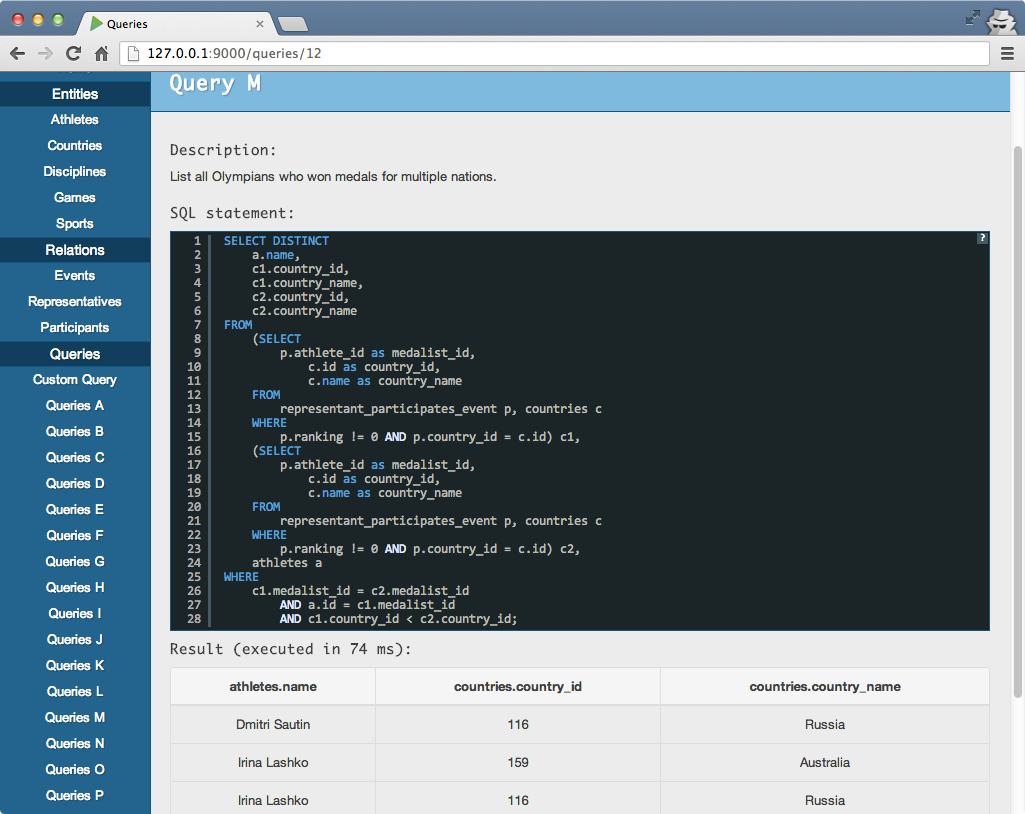
\includegraphics[width=0.9\textwidth]{web3_QueryM}
	\caption{Query view\label{fig:ddl-scheme}}
\end{figure}

\newpage
\section{Add entity / relation}

To change data inside the databases, we can add, edit and remove entities and relations using the WEB UI.

\begin{figure}[!ht]
	\centering
	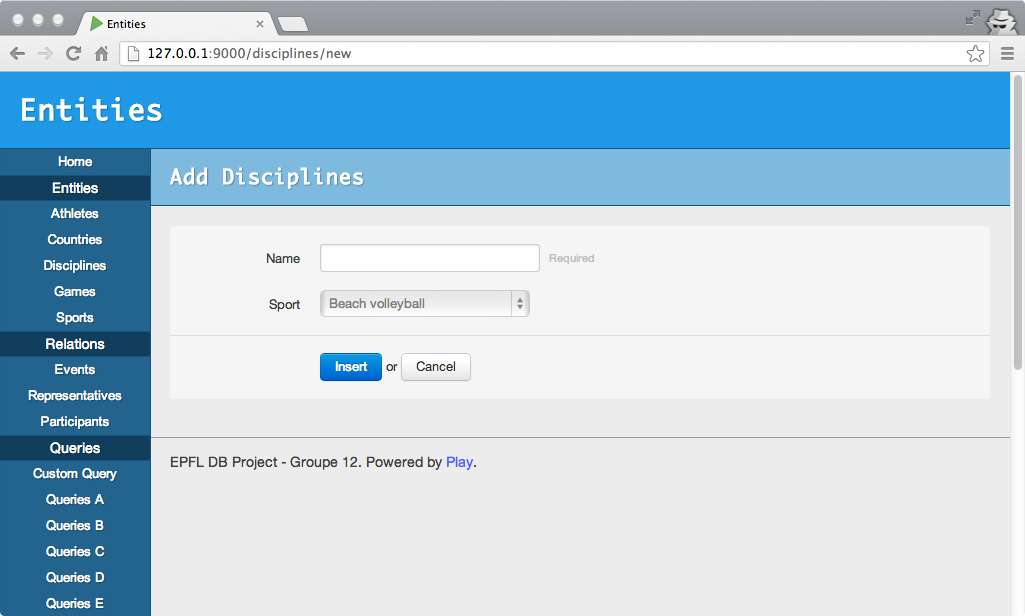
\includegraphics[width=0.9\textwidth]{web3_add}
	\caption{Add entity form\label{fig:ddl-scheme}}
\end{figure}


\section{Custom Query}

To perform custom query, we implement a small interface to insert SQL Code and then query the DB and print the result.
If an error occurs a message is displayed.

\begin{figure}[!ht]
	\centering
	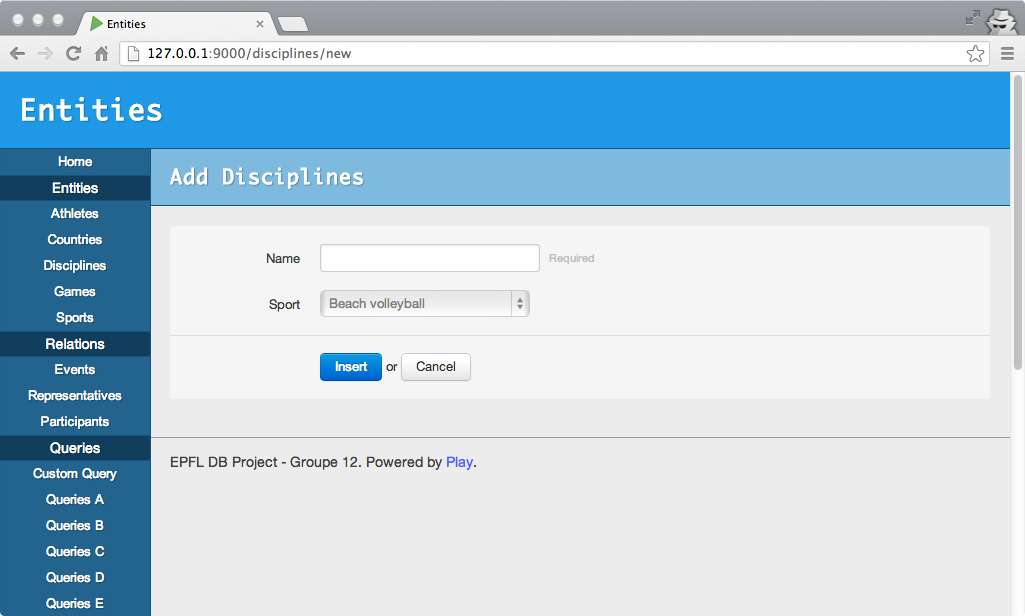
\includegraphics[width=0.9\textwidth]{web3_add}
	\caption{Add entity form\label{fig:ddl-scheme}}
\end{figure}



%------------------------------------------------------------------------------
% END OF DOCUMENT
%------------------------------------------------------------------------------